\subsection{Energy}
The final conserved quantity that we will use to analyze problems is energy. It is the only scalar that we are looking at that is conserved, and is always a positive number. Energy is measured in joules (J), and by definition 1 J = 1 N $\cdot$ m = kg $\cdot$ m$^2$/s$^2$. The rate at which energy is transferred is power and has units of watts (1 W = 1 J/s). 
\subsubsection{Work and Kinetic Energy}
Work is the transfer of energy between objects, and a force is said to do work if the object it is acting upon is displaced, and we might remember it's force times distance - but we need a better definition for work. 
\begin{center}
	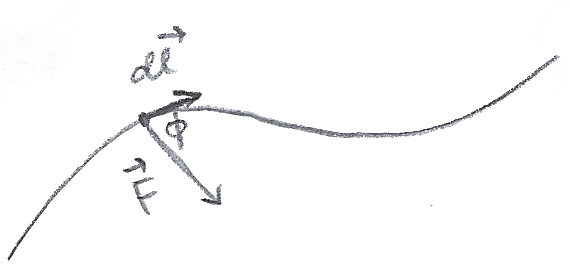
\includegraphics[width=0.3\textwidth]{images/mechintro/work.png}\\
\end{center}
As an object moves along a path while being acted upon by a force, we can split the path into many small displacements. Since work serves to set objects into motion, only the component of the force in the direction of the displacement counts towards the work. So, if the displacement is $d \vec l$, and $\vec F$ is the force, the component of the force in the direction of the displacement is $F \cos \phi$ if $\phi$ is the angle between the displacement and the displacement. This can be written as $\vec F \cdot d\vec l$. Therefore:
\[
	dW = \vec F \cdot d\vec l
\]
where $W$ is the work. For constant force $\vec F$ and linear displacement $d \vec l$ this is true, but to find the total work along any curve $C$, we can let all the little displacements go to zero, let the number of displacements go to infinity and add up all of the little components of work. This is an integral, but a type of integral that we won't encounter in BC Calculus. Somewhat fittingly, this kind of integral is called a line integral, and we can write it as follows:
\[
	W = \int_C \vec F \cdot d\vec l
\]
We won't have to evaluate general line integrals, but for relatively simple cases we will (where the distance is basically linear). \\
This expression for work seems very niche, but we can construct such a line integral from Newton's Second Law, $\vec F = m\vec a = m \dv{\vec v}{t}$. First, we dot the vector on both sides with $\vec v$:
\[
	\vec F \cdot \vec v = m \vec v \cdot \dv{\vec v}{t}
\]
Now, we can integrate with respect to $t$ between times $t_1$ and $t_2$:
\[
	\int_{t_1}^{t_2} \vec F \cdot \vec v \, dt = \int_{t_1}^{t_2} m \vec v \cdot \dv{\vec v}{t} \, dt
\]
The dot product follows the product rule, so I claim that $\frac{1}{2} \dv{}{t}\vec v \cdot \vec v = \vec v \cdot \dv{\vec v}{t}$. Indeed, $\frac{1}{2} \dv{}{t}\vec v \cdot \vec v = \frac{1}{2} \left( \dv{\vec v}{t} \cdot \vec v + \vec v \cdot \dv{\vec v}{t} \right) = \vec v \cdot \dv{\vec v}{t}$. Therefore:
\[
	\int_{t_1}^{t_2} \vec F \cdot \vec v \, dt = \int_{t_1}^{t_2} \frac{1}{2} m \dv{}{t}\vec v \cdot \vec v \, dt = \frac{1}{2} m (\vec v(t_2) \cdot \vec v(t_2) - \vec v(t_1) \cdot \vec v(t_1)) = \frac{1}{2}m (v_{t_2}^2 - v_{t_1}^2 )
\]
The quantity $\frac{1}{2} mv^2$ one might recognize as the kinetic energy $K$ of an object with mass $m$ and velocity $v$, from chemistry. As a refresher, the kinetic energy of an object is the energy the object has that is stored in its movement. This right hand side describes the change in the kinetic energy as the velocity of the object changes during the time interval, so we can write it as $\Delta K$. On the left hand side, since $\dv{\vec l}{t} = \vec v$, $d\vec l = \vec v \, dt$, so we can write the left hand side as an integral along the curve followed by the object during the time interval. In other words, it's our line integral for work! Therefore:
\[
	W = \int_C \vec F \cdot d\vec l = \Delta K
\]
This is the Work-Energy Theorem, which is useful for determining how much work is done to an object after a process by instead measuring its kinetic energy at the beginning and end of the process. \\
As a final sidenote, it's worth noting that kinetic energy has both a translational and rotational form. For an object, a body has translational kinetic energy of $\frac{1}{2}mv^2$, but rotational kinetic energy $\frac{1}{2}I\omega^2$. This expression pops up in the same way when torque is dotted with the angular velocity. Always remember to account for rotational kinetic energy when dealing with rotating objects as well!
\subsubsection{Potential Energy}
Before we introduce the other kind of mechanical energy we'll be studying, potential energy, we have to first introduce the idea of conservative forces versus non-conservative forces. Let's look back at the formula for work: 
\[
	W = \int_C \vec F \cdot d\vec l
\]
For a force $\vec F$, if the work done on the object is independent of the path the object travels, then $\vec F$ is said to be a conservative force. If $\vec F$ does not satisfy this, it is non-conservative. Notice that for $\vec F$ to be conservative, we must have that the work done on an object around a closed loop is zero. Symbolically:
\[
	W = \oint_C \vec F \cdot d\vec l = 0
\]
where the symbol $\oint$ represents integrating around a closed loop (but it's still a line integral). This can be seen by noting that as a particle moves by a conservative force from point $A$ to point $B$, doing some amount of work, the exact negative work is done as the particle moves back from point $B$ to point $A$. With this, we can define the potential energy function $U$ - as work is applied to an object, the potential energy of the object should decrease by the same amount:
\[
	\Delta U = - \int_C \vec F \cdot d\vec l = - W
\]
Usually, potential energy functions are dependent upon the position of the object with respect to the conservative forces at play and give a scalar energy to every point in space, but we'll really only deal with functions in one dimension. The concept is still the same. Also, usually when integrating we'll get a constant - but to simplify things we'll set it to zero, which will sometimes produce negative values of potential energy - but that's fine because it's the relative differences between values that matter more than the actual values. To illustrate this, we'll use an arbitrary one-dimensional conservative force, and look at the potential energy of a particle being acted upon by this force:
\[
	F_x = F_0 \cos \left(\frac{2\pi x}{L} \right)
\]
For the sake of simplicity, both $F_0$ and $L$ have the correct dimensions of force and length, respectively and are both positive.\\ First, let's try to find the potential energy. Consider a path from $x = 0$ to arbitrary $x$ along a straight line. When we do this line integral, then, the dot product basically becomes multiplication, since the force and the displacement are in the same direction, rendering the cosine of the angle between the two to be $1$. Thus, we can calculate $\Delta U$ between these two positions:
\begin{align*}
	\Delta U = U(x) - U_0 &= - \int_C \vec F \cdot d\vec l \\
	&= - \int_0^x  F_0 \cos \left(\frac{2\pi x}{L} \right) \, dx\\
	&= - \frac{F_0L}{2\pi} \sin \left(\frac{2\pi x}{L} \right) \Big|_0^x \\
	&= - \frac{F_0L}{2\pi} \sin \left(\frac{2\pi x}{L} \right)
\end{align*}
If $U_0$ is assumed to be $0$, we can get the not-so-bad-looking function:
\[
	U(x) = - \frac{F_0L}{2\pi} \sin \left(\frac{2\pi x}{L} \right)
\]
This is on the more complex side of potential energy functions we'll be dealing with on a regular basis. The most common ones are the potential energies due to gravity and elastic forces (springs). For these, I'll include them here for you to re-derive. (Note: I'm using $\Delta y$ as a change in the vertical height of an object above the surface of the earth.)
\[
	\vec F = -mg\hat y \quad \Delta U_{grav} = mg\Delta y
\]
\[
	\vec F = -k\Delta x \hat x \quad \Delta U_{spring} = \frac{1}{2}kx^2
\]
\subsubsection{Conservation of Energy}
The fundamental law of the universe is the conservation of mechanical energy $E_{mech}$. We define the mechanical energy of a system $E_{mech}$ to be the sum of the kinetic energy of the system and the potential energy due to all the conservative forces:
\[
	E_{mech} = K_{sys, c} + K_{sys, nc} + U_{sys}
\]
From this, we can observe the following:
\begin{mdframed}[frametitle=Conservation of Mechanical Energy]
If no non-conservative forces act internally in the system, and no external forces put any work into the system, the mechanical energy $E_{mech}$ is constant, and: $$\Delta E_{mech} = \Delta K_{sys} + \Delta U_{sys} = 0$$
More generally, for the universe as a whole, energy cannot be created or destroyed - only converted into other forms.
\end{mdframed}
Notice that if non-conservative forces do act, usually they dissipate energy from the system in the form of heat, a notable example being kinetic friction (static friction does no work). \\
With this in mind, let's revisit the potential energy function that we created in the previous section:
\[
	U(x) = - \frac{F_0L}{2\pi} \sin \left(\frac{2\pi x}{L} \right)
\]
Now, let's launch a particle of mass $m$ from a position with coordinate $x_0$ ($0 < x_0 < \frac{L}{2}$, for simplicity) under the influence of this force. Let's figure out what the maximum velocity of this object is. \\
Intuitively, this can be difficult to imagine. One way we can make this easier for ourselves is to draw an energy diagram. First, we should draw the graph of the potential energy function. In our case, it looks like this:\\
\begin{center}
	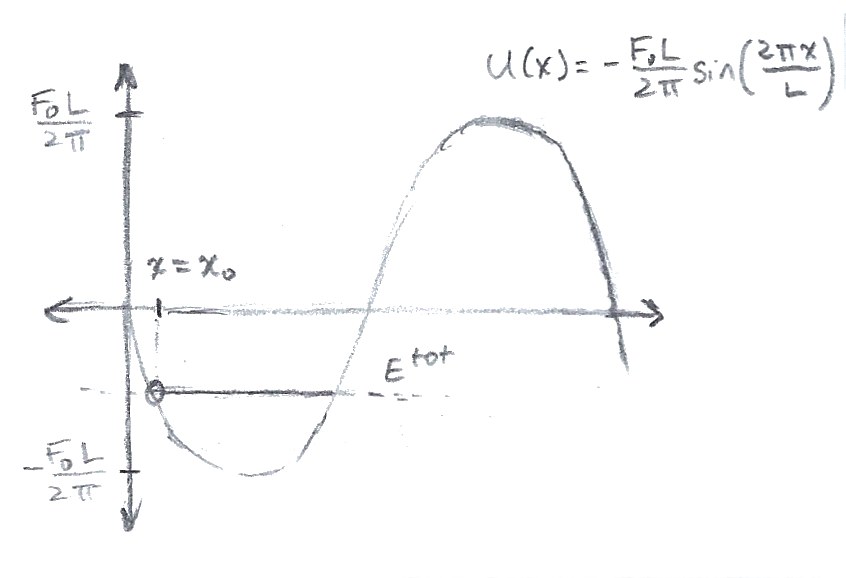
\includegraphics[width=0.5\textwidth]{images/mechintro/cons-energy-1.png}\\
\end{center}
Since there are no external forces on the system and the force is conservative, the energy in the system is conserved. On the graph, we can draw a horizontal line to show how much energy is in the system, as shown. Note that the particle can't reach any position that must cross above the line since otherwise, the system would have more energy than is actually in the system. Therefore, the motion of the particle is restricted to the interval that is bounded by the horizontal line and the potential energy curve. \\
Since potential energy can only be converted to kinetic energy (and vice versa), the particle has its maximum amount of kinetic energy when it has the least amount of potential energy. We can use calculus (or just know how sine functions work, to be honest) to conclude that minimum occurs at $x = \frac{L}{4}$. The potential energy at this point is then:
\[
	U\left(\frac{L}{4}\right) = - \frac{F_0L}{2\pi} \sin \left(\frac{2\pi L}{4L} \right) = - \frac{F_0L}{2\pi}
\]
The change in the potential energy is then:
\[
	\Delta U = U\left(\frac{L}{4}\right) - U(x_0)= \frac{F_0L}{2\pi} \sin \left(\frac{2\pi x_0}{L} \right) - \frac{F_0L}{2\pi}
\]
By conservation of energy, we have $- \Delta U = \Delta K$, so the change in kinetic energy $\Delta K$ is:
\[
	\Delta K = \frac{F_0L}{2\pi}\left(1 - \sin \left(\frac{2\pi x_0}{L} \right)\right)= \frac{1}{2}mv_{max}^2
\]
From this, we get the (pretty messy) expression for the maximum velocity of the particle:
\[
	v_{max} = \sqrt{\frac{F_0L}{\pi m}\left(1 - \sin \left(\frac{2\pi x_0}{L} \right)\right)}
\]
If we launch the particle at some velocity $v_0$, the total energy is higher, because the particle has its own kinetic energy to be accounted for. Let's find the minimum value of $v_0$ for the particle to never return. 
\begin{center}
	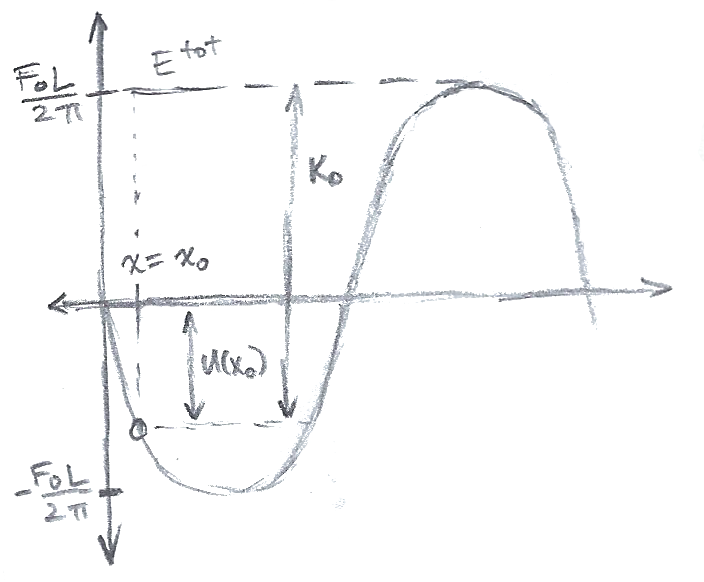
\includegraphics[width=0.4\textwidth]{images/mechintro/cons-energy-2.png}\\
\end{center}
If enough kinetic energy is given to the particle so that it escapes and never comes back to the starting point, the total energy should then be greater than or equal to the maximum value of the potential energy. This means:
\[
	\frac{1}{2}mv_0^2 - \frac{F_0L}{2\pi} \sin \left(\frac{2\pi x_0}{L} \right) = \frac{F_0L}{2\pi}
\]
We can solve and obtain the following expression for $v_0$:
\[
	v_0 = \sqrt{\frac{F_0L}{\pi m} \left(1 + \sin \left(\frac{2\pi x_0}{L} \right) \right)}
\]
The same principles of conservation of energy can be applied to general mechanical systems of a wide variety, as will be seen in the problems.  
\subsubsection{Summary and Problems}
The conservation of energy is a useful principle that can be applied widely to many problems where other dynamical information may not be available. In particular, it tends to provide a helpful link between velocity and position that is not readily attainable from momentum, dynamics, or kinematics. These problems may integrate concepts from all the other units as well - including collisions, which can be classified as elastic, completely inelastic, or partially inelastic. Elastic collisions conserve kinetic energy of the objects before and after the collision, completely inelastic collisions occur when the objects have the same velocity, and partially inelastic collisions satisfy neither of these conditions. Most problems that we will see will either concern a completely inelastic or elastic collision. As a final general rule of thum, remember that if energy is not conserved during a process, be sure to note where that energy goes, whether if it's lost to nonconservative forces such as friction or in a collision. \\

\noindent \textbf{Problems:}\\
1. (2 $\bigstar$) A box slides from rest down a frictionless ramp inclined at an angle $\theta$ with respect to the horizontal and is stopped at the bottom of the ramp by a spring with a spring constant of $k$. If the box has a mass of $m$ and slides a distance $d$ from the point of release to the point where it comes to rest against the spring, show the compression $x$ of the spring when the box comes to rest is $x = \sqrt{\frac{2mgd\sin\theta}{k}}$.\\
2. (3 $\bigstar$) A child of mass $m$ on a playground swing moves with a speed of $v_0$ when the swing of length $L$ is at its lowest point. Show that the angle $\theta$ that the swing makes with the vertical when the child is at the highest point is equal to $\theta = \arccos\left(1- \frac{v_0^2}{2gL}\right)$.\\
3. (3 $\bigstar$) A pendulum consists of a small bob of mass m attached to a string of length $L$. The bob is held to the side with the string horizontal. Then the bob is released from rest. At the lowest point of the swing, the string catches on a thin peg a distance $R$ above the lowest point. Show that $R$ must be smaller than $2L/5$ if the string is to remain taut as the bob swings around the peg in a full circle. \\
4. (2 $\bigstar$)  A small object of mass $m$ moves in a horizontal circle of radius $r$ on a rough table. It is attached to a horizontal string fixed at the center of the circle. The speed of the object is initially $v_0$. After completing one full trip around the circle, the speed of the object is $0.5v_0$. a) Show that the energy dissipated by friction during that one revolution is $\frac{3}{8}mv_0^2$. b) Show that the coefficient of kinetic friction is $\frac{3v_0^2}{16\pi gr}$. c) Show that the object will make a further $\frac{1}{3}$ of a revolution before coming to rest.\\
5. (3 $\bigstar$, $\spadesuit$) The potential energy of a diatomic molecule is given by the following expression with $r$ being the separation of the two atoms of the molecule and $A$ and $B$ being positive constants: $$U = A/r^{12} - B/r^6$$ This potential energy is associated with the force that binds the two atoms together. Show that the equilibrium distance $r$ where no net force acts on either molecule is $1.12(A/B)^{1/6}$.\\
6. (4 $\bigstar$) A pendulum consists of a compact 0.60 kg bob attached to a string of length 1.00 m. A block of mass $m$ rests on a horizontal frictionless surface. The pendulum is released from rest at an angle of 53$^\circ$ with the vertical. The bob collides elastically with the block at the lowest point in its arc. Following the collision, the maximum angle of the pendulum with the vertical is 5.73$^\circ$. Show that the mass $m$ can be equal to both 0.751 kg and 0.479 kg. \\
7. (3 $\bigstar$) A neutron of mass $m$ makes an elastic head-on collision with a stationary nucleus of mass $M$. a) Show that the kinetic energy of the nucleus after the collision is given by $K_{nucleus} = \frac{4Mm}{(m+M)^2}K_n$ where $K_n$ is the initial kinetic energy of the neutron. b) Show that the fractional change in the kinetic energy of the neutron is given by $\frac{\Delta K_n}{K_n} = -\frac{4(m/M)}{1+(m/M)^2}$.
\pagebreak